De interlace eigenschap van een tridiagonale, symmetrische en re\"ele matrix $A$ luidt als volgt. Voor $A \in \mathbb{R}^{n \times n}$, en $A^{(1)}, A^{(2)}  \dots A^{(n)}$ de principale vierkante submatrices van dimensie $1, 2 \dots n$, geldt dat de eigenwaarden van deze submatrices interlacen. Dit wil zeggen dat $\lambda_j^{(k+1)} \leq \lambda_j^{(k)} \leq \lambda_{j+1}^{(k+1)}$. Als $A$ irreduceerbaar is (en dus geen nul heeft op een nevendiagonaal), dan worden de ongelijkheden strikte ongelijkheden. Dit laatste is belangrijk voor de bisectie-methode.

Als voorbeeld nemen we de tridiagonale, symmetrische en re\"ele matrix
$$A = \begin{bmatrix} 
1 &5 &0 &0\\
5 &2 &6 &0 \\
0 &6 &3 &7\\
0 &0 &7 &4
\end{bmatrix}.$$
We zien duidelijk op figuur \ref{fig:oef9_1} dat de eigenwaarden van een principale submatrix tussen de eigenwaarden van de principale submatrix van een dimensie groter liggen.

\begin{figure}[H]
    \centering
    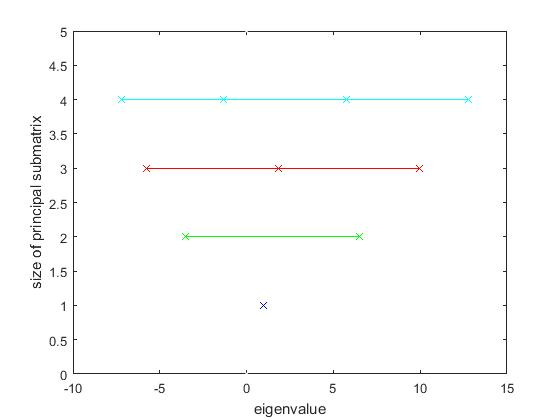
\includegraphics[width=0.7\textwidth]{oef9_1.jpg}
    \caption{De eigenwaarden van de opeenvolgende principale submatrices van A}
    \label{fig:oef9_1}
\end{figure}